\section{Gleichstromumrichter}
Ein Gleichstromumrichter dient zur Änderung von: \textbf{Polarität, Spannung, Strom}.\newline
\vspace{-0.2cm}
\[ \tau=\frac{L_1}{R_1} \qquad T_s=T_{on} + T_{off} \qquad  D = \frac{U_2}{U_1}=\frac{I_1}{I_2}=\frac{t_{on}}{T_s} \]
\vspace{-1cm}
\subsection{Buck-Converter}
\begin{minipage}{0.75\linewidth}
    Tiefsetzsteller (Buck-Converter) $U_a < U_e  $\newline
    \textbf{Rechnung ohne C}\newline
    \renewcommand{\arraystretch}{2}
    \begin{tabular}{p{9cm} p{3cm}}
        $ V_1 = i_L\cdot R_1+L_1\cdot\frac{\diff i_L}{\diff t} $ &
        $ 0<t<T_{on} $
        \\  
        $ 0 = i_L\cdot R_1+L_1\cdot\frac{\diff i_L}{\diff t}$ & $T_{on}<t<T_{s} $
        \\  
        $ i_L=\frac{V_1}{R_1}+ \frac{V_1}{R_1}\cdot \frac{e^{-\frac{T_{off}}{\tau}}-1}{1-e^{-\frac{T_{s}}{\tau}}}\cdot e^{-\frac{t}{\tau}}$ &
        $ 0<t<T_{on}  $
        \\  
        $ i_L=\frac{V_1}{R_1}\cdot \frac{1-e^{-\frac{T_{on}}{\tau}}}{1-e^{-\frac{T_{s}}{\tau}}}\cdot e^{-\frac{t-T_{on}}{\tau}}$ &
        $ T_{on}\leq t \leq T_{s}  $
        \\ 
        $ i_{Lmax} = i_L(T_{on}) \qquad i_{Lmin} = i_L(0) = i_L(T_s) $    
        & \\ 
        $ T_{off}=-\tau \cdot ln\frac{i_{Lmin}}{i_{Lmax}}= -\frac{L_1}{R_1}\cdot ln\frac{i_{Lmin}}{i_{Lmax}} $
        & \\    
        $ T_{on}=-\tau \cdot ln\left(\dfrac{\frac{1}{i_{Lmax}}\cdot\frac{V_1}{R_1}-1}{\frac{1}{i_{Lmax}}\cdot \frac{V_1}{R_1}-e^{-\frac{T_off}{\tau}}}\right) $
        & \\ 
        $ V_{out}=V_{in}\cdot \frac{T_{on}}{T_{on}+T_{off}}-V_D\cdot\frac{T_{off}}{T_{on}+T_{off}} $
        & \\ 
    \end{tabular}
\newline
\textbf{Übung 6 Gleichstrom Umrichter $ \rightarrow $ Buck-Converter}
\renewcommand{\arraystretch}{1}
\end{minipage}
\begin{minipage}{0.25\linewidth}
    \vspace{-3cm}
    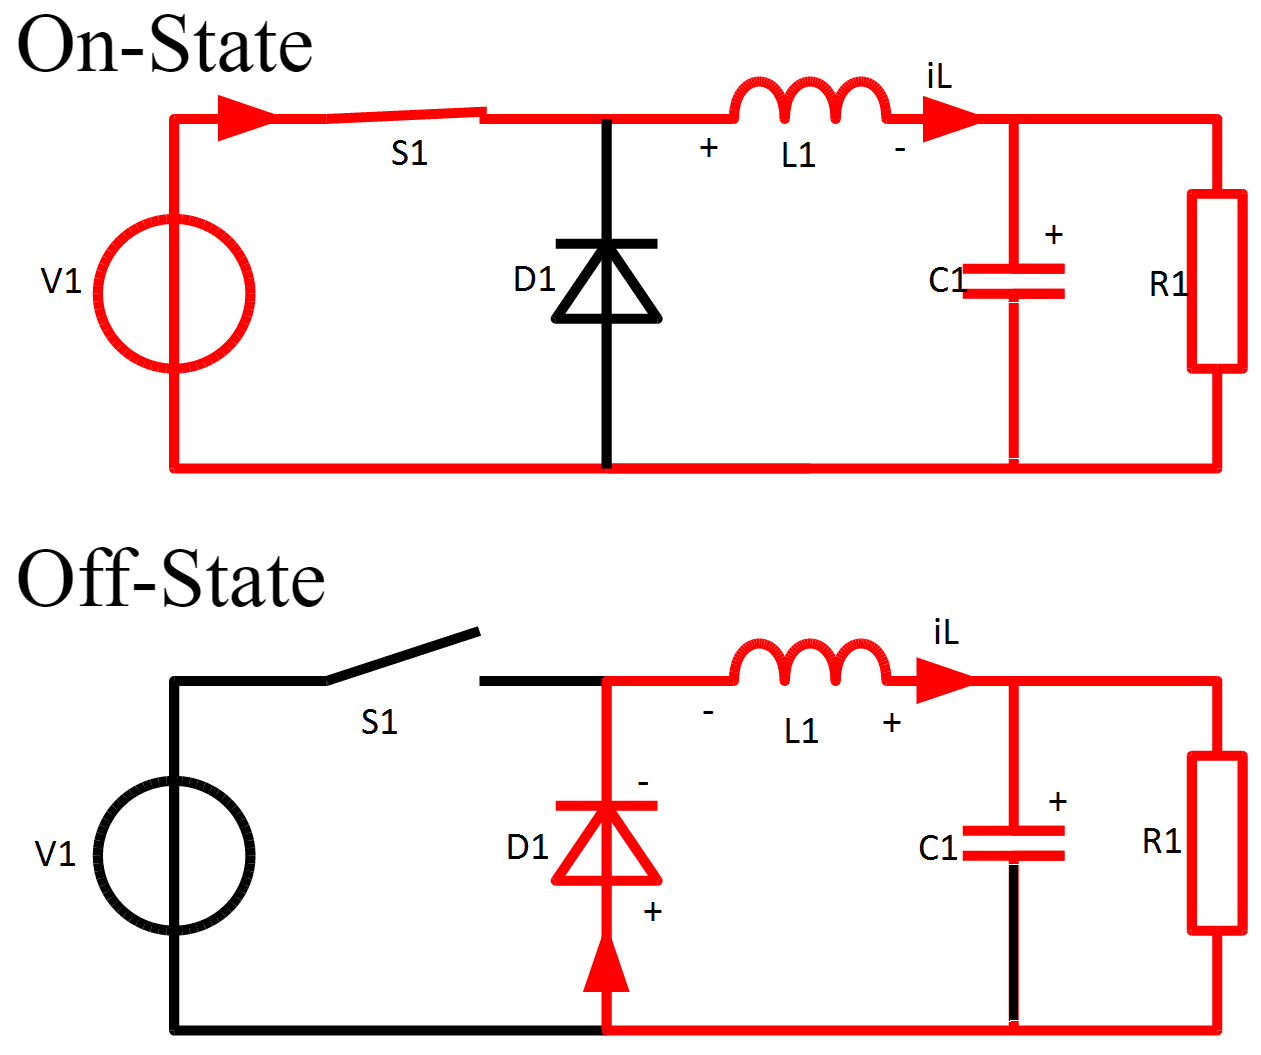
\includegraphics[width=\linewidth]{images/BuckOnOff}
    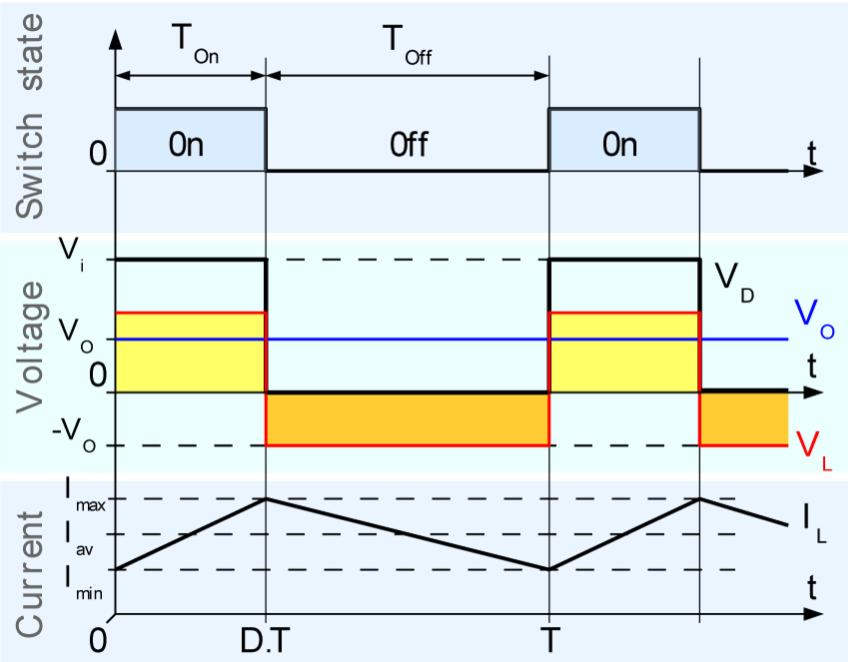
\includegraphics[width=\linewidth]{images/BuckSwitch}
\end{minipage}
\vspace{-0.5cm}
\subsection{Boost-Converter}
\begin{minipage}{0.75\linewidth}
    Hochsetzsteller (Boost-Converter) $U_a > U_e  $\newline
    \[ V_{Out}=V_{in}\cdot \left(1+\frac{T_{on}}{T_{off}} \right)\]
    
\end{minipage}
\begin{minipage}{0.25\linewidth}
    \vspace{-3cm}
    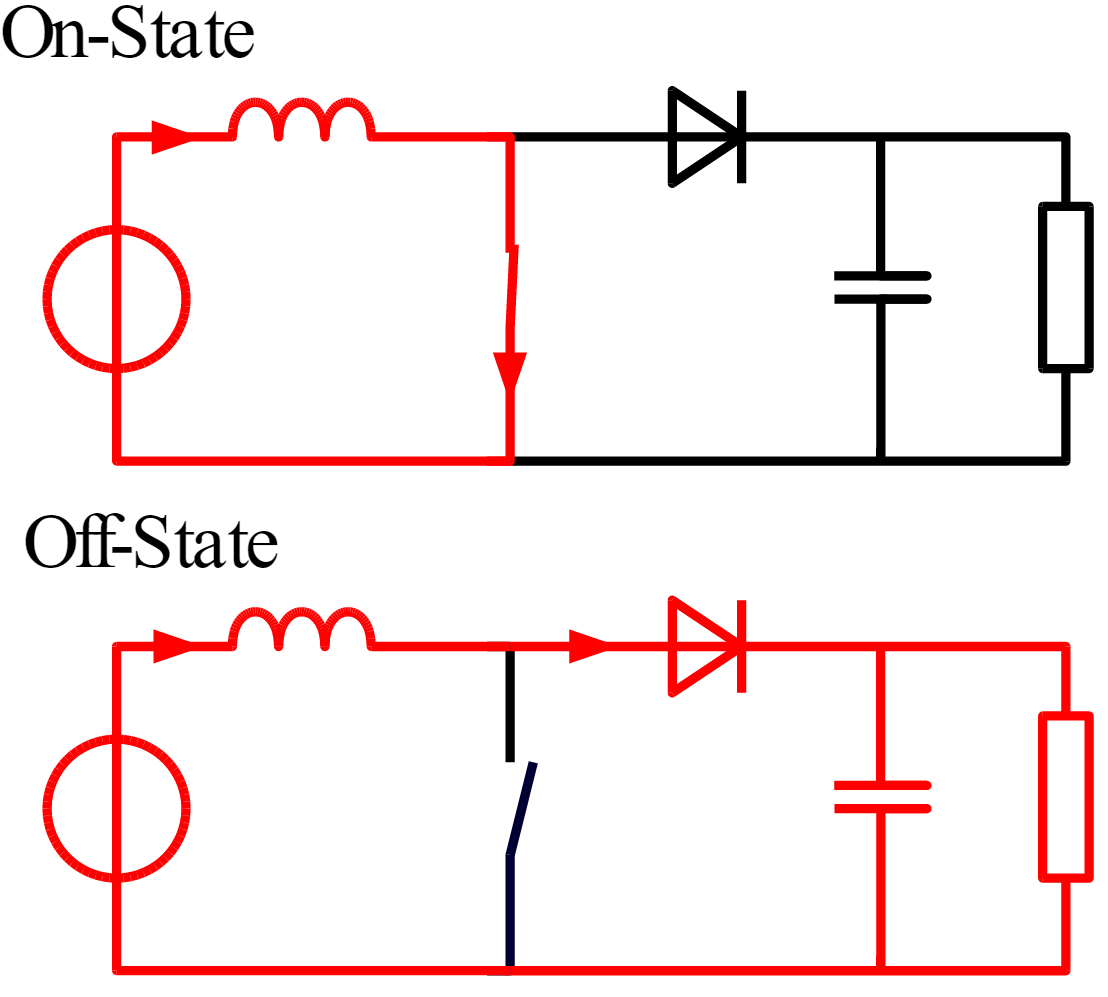
\includegraphics[width=\linewidth]{images/BoostOnOff}
    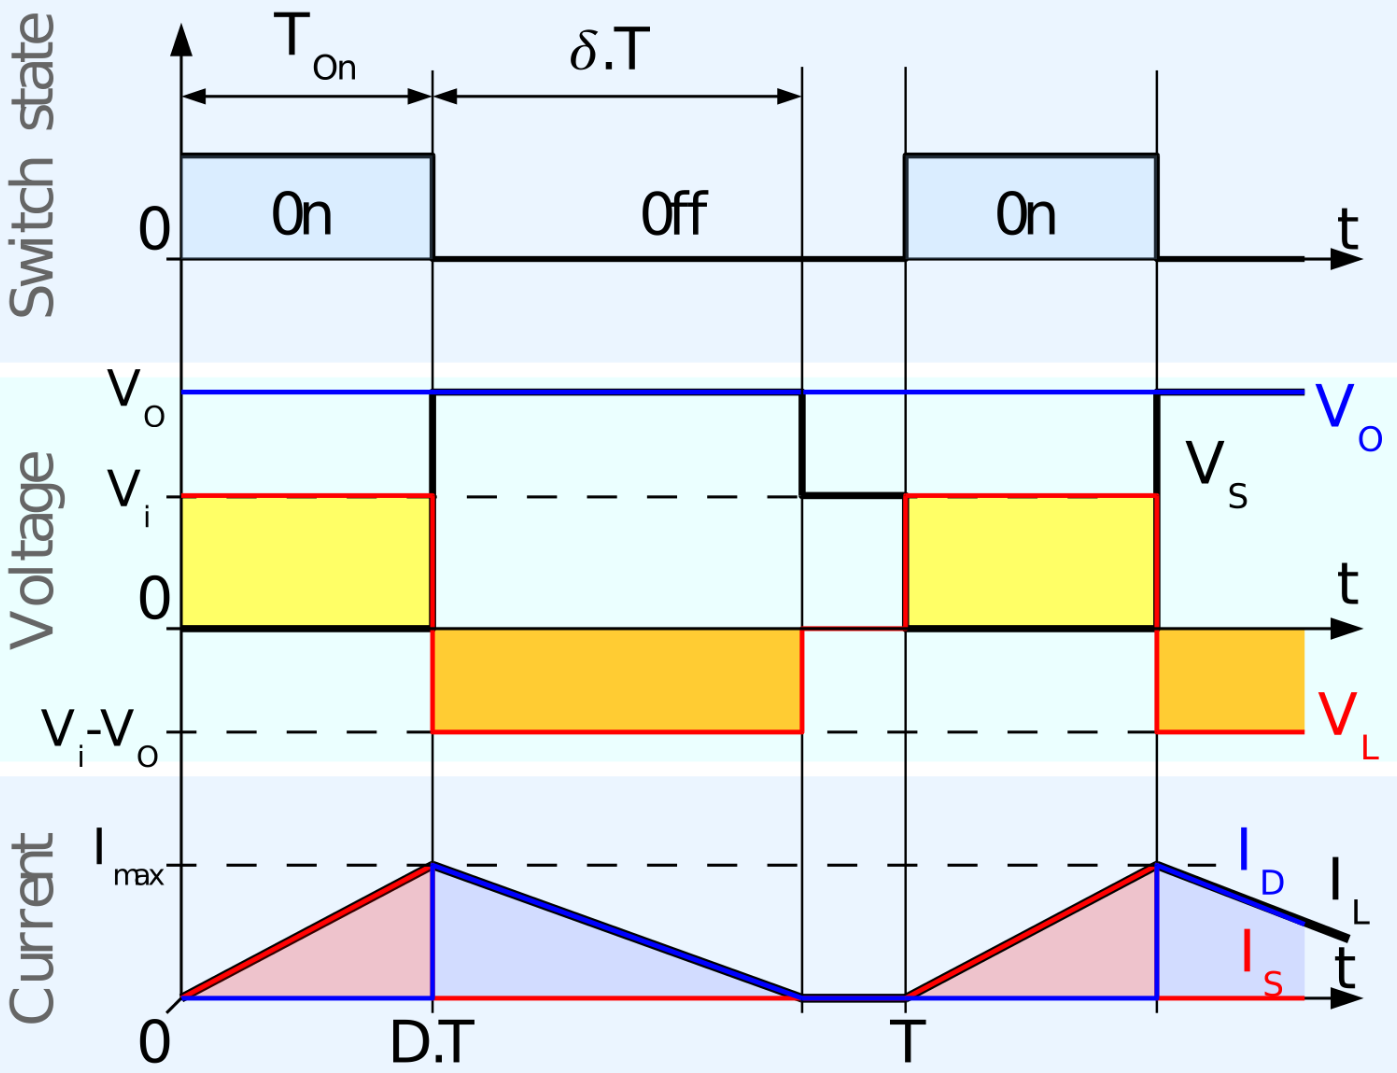
\includegraphics[width=\linewidth]{images/BoostSwitch}
\end{minipage}

\subsection{Inverse-Converter}
\begin{minipage}{0.75\linewidth}
Inverswandler, Umkehrung der Polarität\newline
\[ V_{out}=-L\cdot \frac{\varDelta I_L }{\varDelta t} \overbrace{=}^{eingeschwungen}V_L \cdot \frac{T_{on}}{T_{off}} \]
\end{minipage}
\begin{minipage}{0.25\linewidth}
    \vspace{-3cm}
    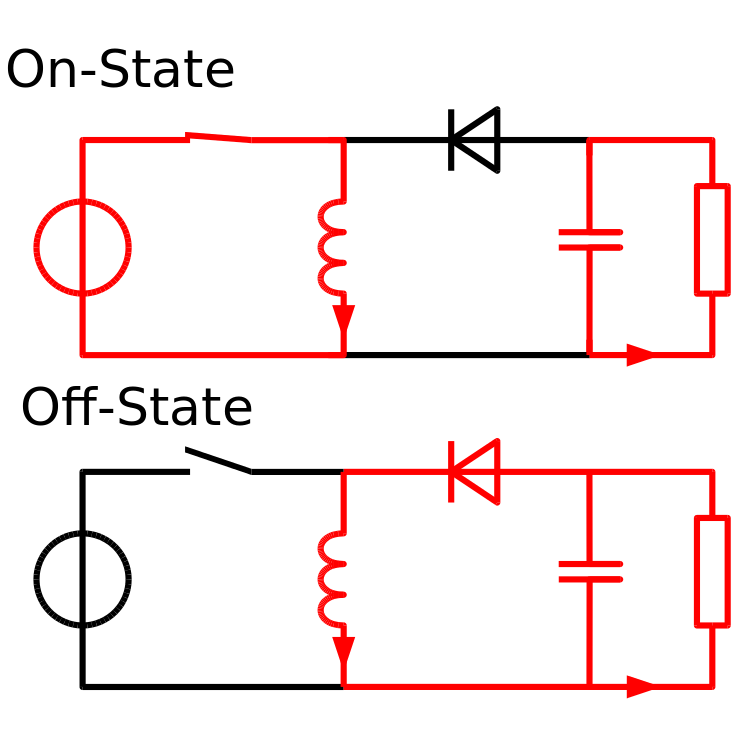
\includegraphics[width=\linewidth]{images/InverseOnOff}
    \includegraphics[width=\linewidth]{images/InverseSwitch}
\end{minipage}

\subsection{Gleichstromschalter/Gleichstromsteller}
\subsubsection{Gleichstromschalter}
\begin{minipage}{0.5\linewidth}
    \textbf{Nur Einschalten}\newline
    \[ U_1=(L + L_{\sigma})\cdot \frac{\diff i_L}{\diff t}+R\cdot i_L \]
    \[ i_L(t)=\frac{U_1}{R}\cdot(1-e^{-\frac{t-t_{on}}{\tau}})\]
\end{minipage}
\begin{minipage}{0.4\linewidth}
    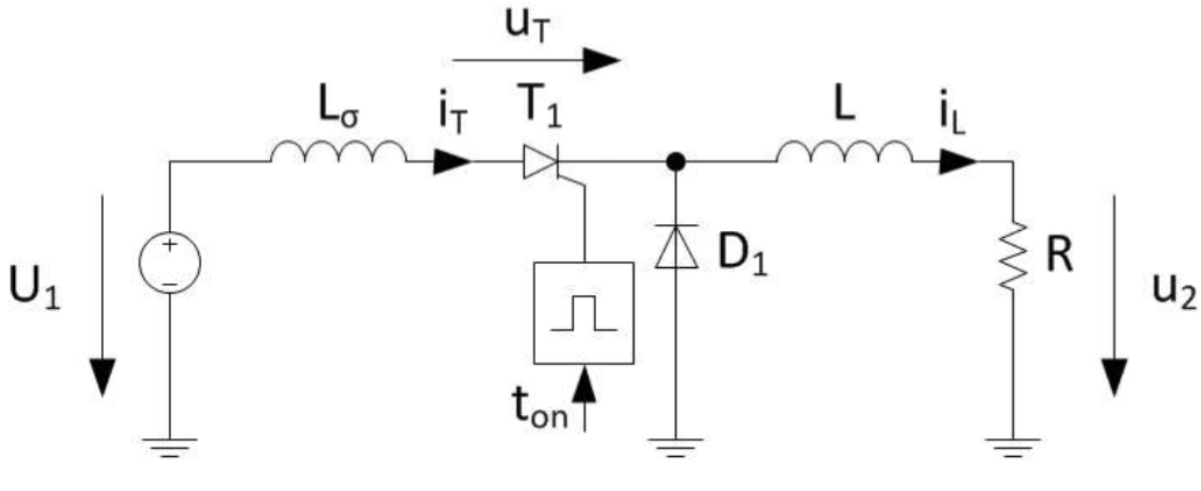
\includegraphics[width=1.2\linewidth]{images/GsSchalterOn}
\end{minipage}

\begin{minipage}{0.5\linewidth}
\textbf{Ein- und Ausschalten}\newline
\[ U_1=(L + L_{\sigma})\cdot \frac{\diff i_L}{\diff t}+R\cdot i_L \qquad t_{on} \leq t \leq t_{off}\]
\[ 0=L\cdot \frac{\diff i_L}{\diff t}+ R\cdot i_L \qquad \qquad \quad t_{off}\leq t \]
\[ i_L(t)=\frac{U_1}{R}\cdot(1-e^{-\frac{t-t_{on}}{\tau}}) \qquad \quad t_{on} \leq t \leq t_{off}\]
\[ i_L(t)=\frac{U_1}{R}\cdot e^{-\frac{t-t_{off}}{\tau}} \qquad \quad \qquad t_{off}\leq t \]
\end{minipage}
\begin{minipage}{0.4\linewidth}
    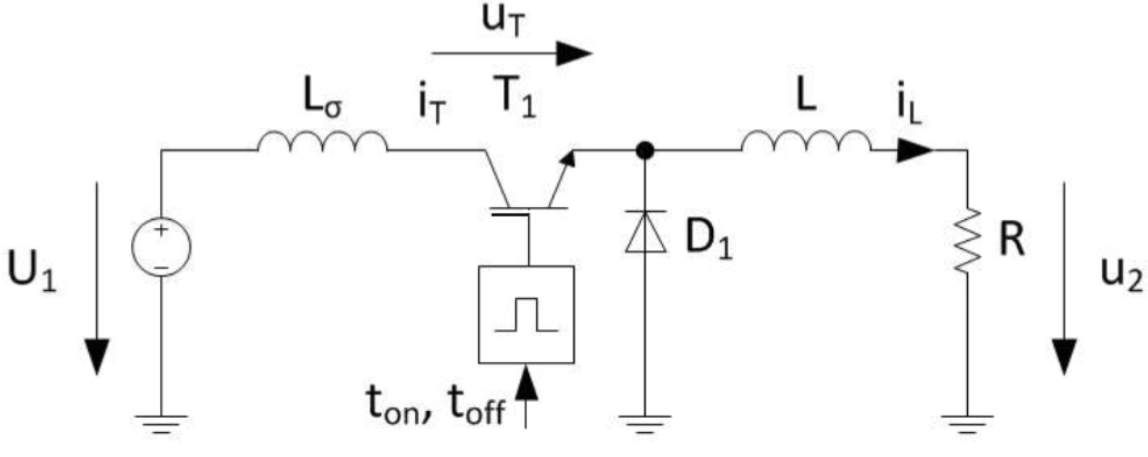
\includegraphics[width=1.2\linewidth]{images/GsSchalterOnOff}
\end{minipage}

\subsubsection{Gleichstromsteller}
\begin{minipage}{0.5\linewidth}
\[ U_{2AV}=\frac{1}{t_{on}+t_{off}}\int_{0}^{t_e}U_1\cdot \diff t = \frac{t_{on}}{t_{on}+t_{off}}U_1 \]
\end{minipage}
\begin{minipage}{0.4\linewidth}
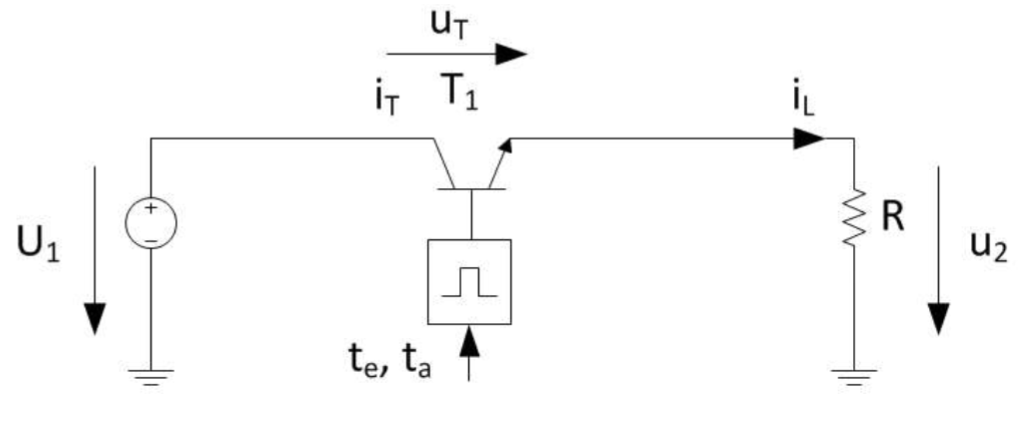
\includegraphics[width=1.2\linewidth]{images/GsSteller}
\end{minipage}

\begin{minipage}{0.5\linewidth}
    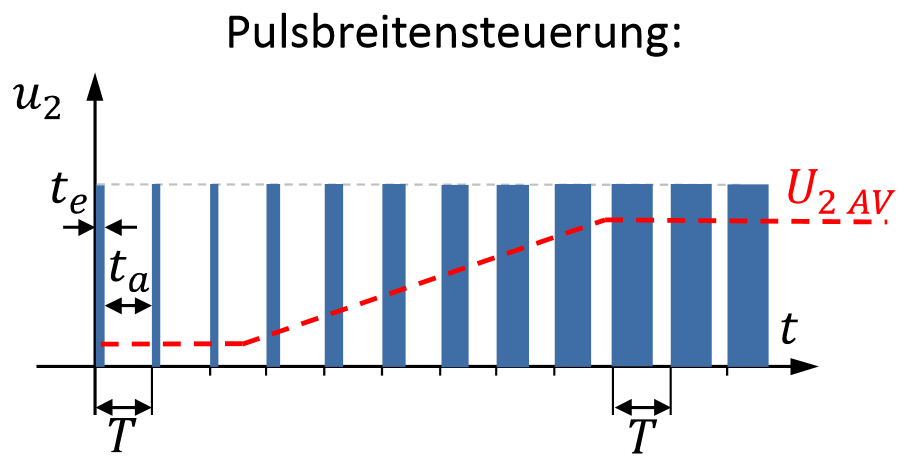
\includegraphics[width=0.8\linewidth]{images/GsStellerPuls}
\end{minipage}
\begin{minipage}{0.5\linewidth}
    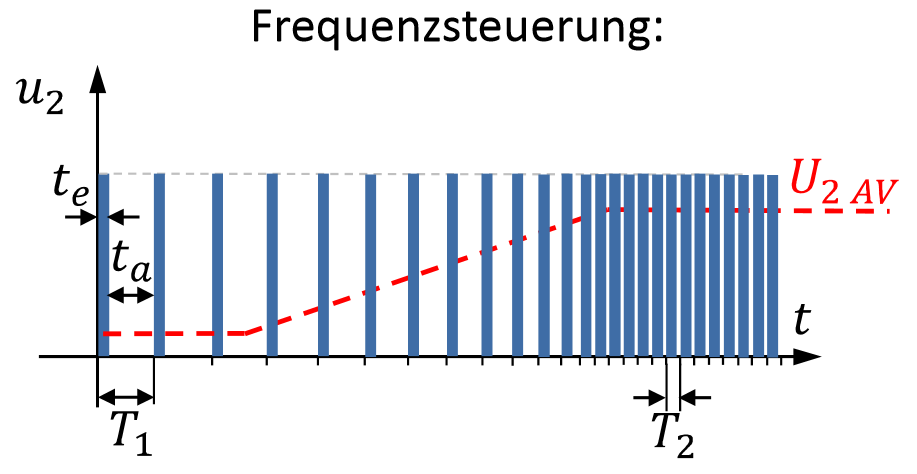
\includegraphics[width=0.8\linewidth]{images/GsStellerFreq}
\end{minipage}

\textbf{Ein-Quadranten-Betrieb}\newline
\begin{minipage}{0.7\linewidth}
    \begin{longtable}{   p{.50\textwidth}  p{.6\textwidth} }
         $U_{m2} = \frac{T_E}{T}\cdot U_D = F_p\cdot T_E \cdot U_D$ &
         $U_{m2}$ = Mittelwert Ausgangsspg.\newline
         $T_e $ = Einschaltzeit \newline
         $T$ = Periodendauer \newline
         $U_D$ = Zwischenkreisspg. \newline
         $f_q$ = Freq
         \\  
         
         $\varDelta i_2 = 2 \alpha\frac{U_D}{L}T_E(1-\frac{T_E}{T})$ &
         $\alpha$ = 0.5 \quad 1Q-Betrieb \newline
         $\alpha$ = 1 \quad MehrQ-Betrieb
         \\
         
         $ P = U_D I_{m2}\frac{T_E}{T} $&
         $i_2$ =Ausgangsstrom\newline
         $i_{m2}$ = Mittelwert Ausgansstr.\newline
         $L$ = ind. der Last \newline
         $P$ = Ausgangsleistung
         \\
         
         $U_{ac\; 2}=\sqrt{U_2^2-U_{m2}^2}= U_D\sqrt{\frac{T_E}{T}(1-\frac{T_E}{T})} $ &
         $U_{ac2}$= Wechselstromkomponente von U ist\newline
         maximal bei Tastgrad 50\% \\        
    \end{longtable}
\end{minipage}
\begin{minipage}{0.3\linewidth}
    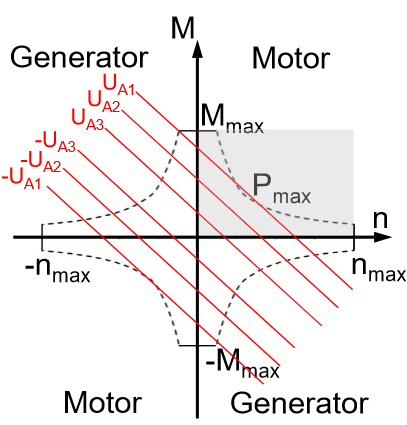
\includegraphics[width=0.8\linewidth]{images/GsSteller1Q}
\end{minipage}

\clearpage